\subsection{Experimentación}

En esta sección se presentan los experimentos realizados para evaluar el rendimiento del algoritmo de Iteración de Valor en el entorno. Se analiza cómo diferentes parámetros del algoritmo afectan su capacidad para encontrar políticas óptimas, su convergencia y su eficiencia.

\subsubsection{Experimento factor de descuento \& umbral de convergencia}

\paragraph{Diseño experimental}
El objetivo de este experimento es analizar cómo los parámetros factor de descuento (\(\gamma\)) y umbral de convergencia (\(\epsilon\)) afectan el rendimiento del algoritmo de iteración de valor.

% TODO: Usar esta tabla para cada experimento
\begin{table}[H]
    \centering
    \begin{tabularx}{\textwidth}{|p{4cm}|X|} % Especificar el ancho de las columnas
        \hline % Línea horizontal superior
        \textbf{Observación} & El rendimiento y óptimalidad de la política encontrada por \textit{Value Iteration} se ven afectados por los valores de $\gamma$ y $\epsilon$.
        \\ \hline
        \textbf{Planteamiento} & Para cada pareja de valores de $\gamma$ y $\epsilon$, se compara la tasa de acierto (llegar al estado final), la recompensa media, número de pasos y tiempo de entrenamiento del algoritmo.
        \\ \hline
        \textbf{Hipótesis} & Se espera que un mayor valor de $\gamma$ conduzca a una política más óptima, mientras que un menor valor de $\epsilon$ permita una convergencia más rápida con una menor precisión.
        \\ \hline
        \textbf{Método} & 
        \begin{itemize}
            \item Se elige un conjunto de valores para $\gamma$ y $\epsilon$: \(\gamma \in \{0.5, 0.7, 0.9, 0.95, 0.99\}\) y \(\epsilon \in \{1\times 10^{-1}, 1\times 10^{-2}, 1\times 10^{-4}, 1\times 10^{-8}\}\).
            \item Para cada combinación de \(\gamma\) y \(\epsilon\), se ejecuta el algoritmo \textit{Value Iteration} en el entorno.
            \item Se evalúa la política obtenida probándola con 500 episodios.
            \item A diferencia de otros algoritmos que requieren de múltiples ejecuciones por su naturaleza estocástica, para Value Iteration basta con una única ejecución por combinación de parámetros, ya que es un algoritmo determinista que siempre converge a la misma política óptima para unos valores dados de $\gamma$ y $\epsilon$.
        \end{itemize}
        \\ \hline
    \end{tabularx}
    \caption{Value Iteration - Experimento 1 - Factor de descuento \& umbral de convergencia}
    \label{tab:diseñoValueIterationExp1}
\end{table}

\newpage

\paragraph{Resultados}

A continuación se presenta un análisis detallado de las diferentes métricas evaluadas en el experimento. La Tabla \ref{tab:resultadosValueIteration} muestra un resumen de los resultados más relevantes:

\begin{table}[H]
    \centering
    \begin{tabular}{|c|c|c|c|c|c|}
        \hline
        $\gamma$ & $\epsilon$ & Tasa éxito & Recompensa & Pasos & Tiempo (s) \\
        \hline
        0.99 & $10^{-8}$ & 1.000 & -63.422 & 63.4 & 31.77 \\
        0.95 & $10^{-4}$ & 1.000 & -64.190 & 64.2 & 13.74 \\
        0.90 & $10^{-2}$ & 1.000 & -63.920 & 63.9 & 7.24 \\
        0.70 & $10^{-1}$ & 0.666 & -144.702 & 144.7 & 2.44 \\
        0.50 & $10^{-1}$ & 0.594 & -152.758 & 152.8 & 1.61 \\
        \hline
    \end{tabular}
    \caption{Resultados representativos del experimento con Value Iteration}
    \label{tab:resultadosValueIteration}
\end{table}

\textbf{Tasa de éxito}

La Figura \ref{fig:successRateValueIteration} muestra la tasa de éxito para las diferentes combinaciones de parámetros:

\begin{itemize}
    \item Valores altos de $\gamma$ ($\geq 0.9$) logran tasas de éxito perfectas (100\%) o casi perfectas.
    \item Con $\gamma = 0.7$:
    \begin{itemize}
        \item 100\% de éxito con $\epsilon \leq 10^{-4}$
        \item Cae al 89.6\% con $\epsilon = 10^{-2}$
        \item Solo 66.6\% con $\epsilon = 10^{-1}$
    \end{itemize}
    \item Con $\gamma = 0.5$:
    \begin{itemize}
        \item 100\% de éxito solo con $\epsilon = 10^{-8}$
        \item Deterioro progresivo: 96.4\% ($10^{-4}$), 77.4\% ($10^{-2}$), 59.4\% ($10^{-1}$)
    \end{itemize}
\end{itemize}

\begin{figure}[H]
    \centering
    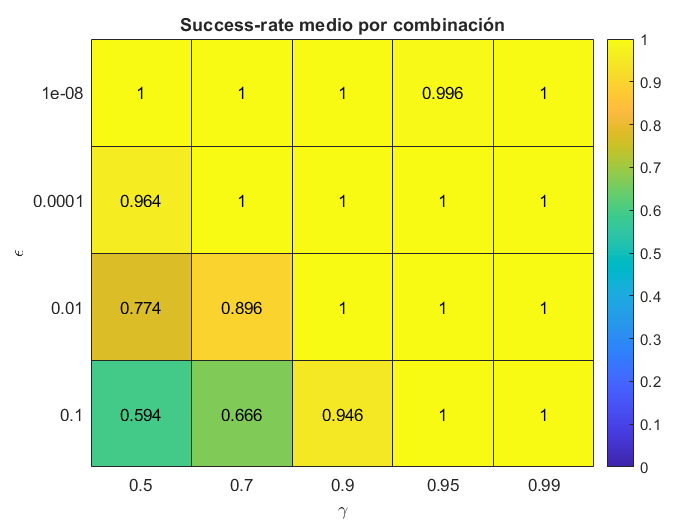
\includegraphics[width=0.7\textwidth]{../../experiments/valueIteration/experiment-1/results/success.png}
    \caption{Tasa de éxito para diferentes valores de $\gamma$ y $\epsilon$ en el algoritmo de iteración de valor.}
    \label{fig:successRateValueIteration}
\end{figure}

\textbf{Recompensa media}

\begin{figure}[H]
    \centering
    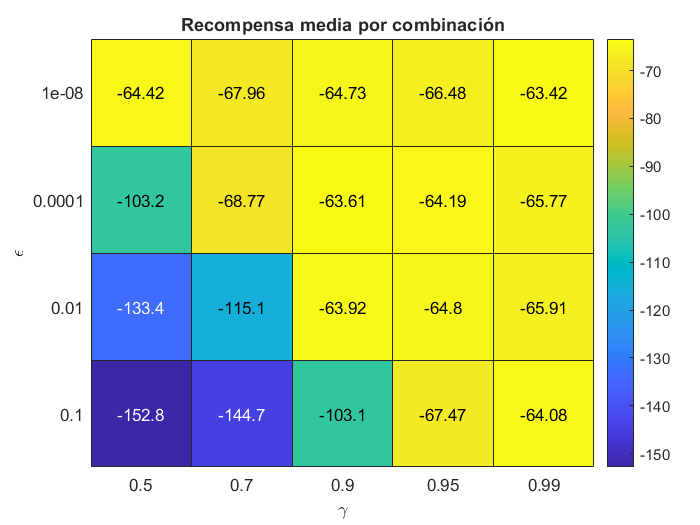
\includegraphics[width=0.7\textwidth]{../../experiments/valueIteration/experiment-1/results/reward.png}
    \caption{Recompensa media para diferentes valores de $\gamma$ y $\epsilon$.}
    \label{fig:rewardValueIteration}
\end{figure}

El análisis de las recompensas medias muestra patrones claros:

\begin{itemize}
    \item Con $\gamma = 0.99$:
    \begin{itemize}
        \item Mejor recompensa global (-63.422) con $\epsilon = 10^{-8}$
        \item Rendimiento consistente en todo el rango de $\epsilon$: -65.766 ($10^{-4}$), -65.906 ($10^{-2}$), -64.080 ($10^{-1}$)
    \end{itemize}
    \item Con $\gamma = 0.9$:
    \begin{itemize}
        \item Recompensas similares con $\epsilon \leq 10^{-2}$: -64.734 ($10^{-8}$), -63.608 ($10^{-4}$), -63.920 ($10^{-2}$)
        \item Deterioro significativo con $\epsilon = 10^{-1}$: -103.114
    \end{itemize}
    \item Valores bajos de $\gamma$:
    \begin{itemize}
        \item $\gamma = 0.7$: recompensas entre -67.962 y -144.702
        \item $\gamma = 0.5$: peor rendimiento, llegando a -152.758 con $\epsilon = 10^{-1}$
    \end{itemize}
\end{itemize}

\newpage

\textbf{Número de pasos}

\begin{figure}[H]
    \centering
    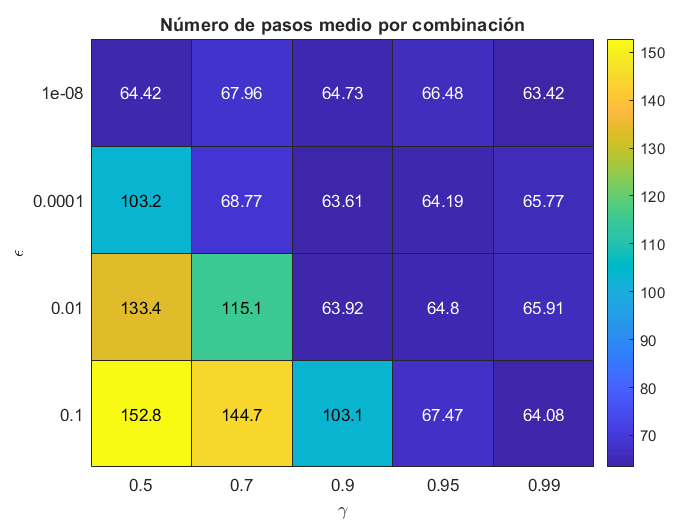
\includegraphics[width=0.7\textwidth]{../../experiments/valueIteration/experiment-1/results/steps.png}
    \caption{Número medio de pasos para diferentes valores de $\gamma$ y $\epsilon$.}
    \label{fig:stepsValueIteration}
\end{figure}

El análisis de los pasos necesarios revela patrones similares a las recompensas:

\begin{itemize}
    \item Mejores resultados con $\gamma \geq 0.9$:
    \begin{itemize}
        \item $\gamma = 0.99$: consistentemente eficiente (63.4-65.9 pasos)
        \item $\gamma = 0.95$: rendimiento similar (64.2-67.5 pasos)
        \item $\gamma = 0.90$: eficiente con $\epsilon \leq 10^{-2}$ (63.6-64.7 pasos)
    \end{itemize}
    \item Deterioro con valores bajos de $\gamma$:
    \begin{itemize}
        \item $\gamma = 0.7$: aumento significativo (68.0-144.7 pasos)
        \item $\gamma = 0.5$: peor rendimiento (64.4-152.8 pasos)
    \end{itemize}
    \item Efectos de $\epsilon$:
    \begin{itemize}
        \item Mayor impacto en $\gamma$ bajos
        \item Menor influencia en $\gamma$ altos ($\geq 0.9$)
    \end{itemize}
\end{itemize}

\newpage

\textbf{Tiempo de entrenamiento}

\begin{figure}[H]
    \centering
    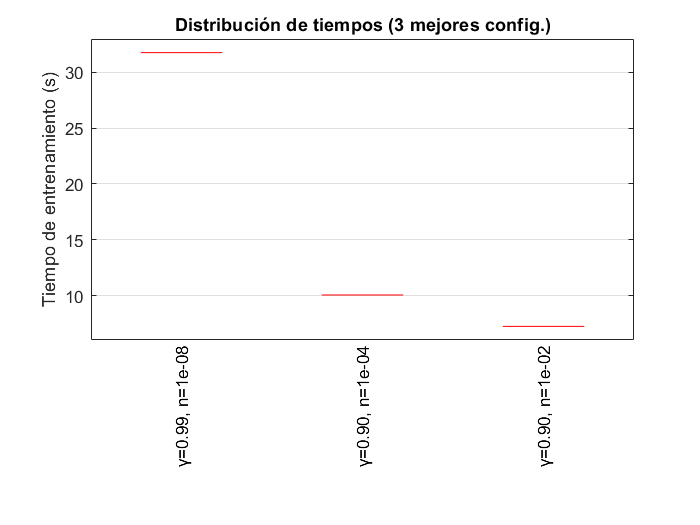
\includegraphics[width=0.7\textwidth]{../../experiments/valueIteration/experiment-1/results/time.png}
    \caption{Tiempo de entrenamiento para diferentes valores de $\gamma$ y $\epsilon$.}
    \label{fig:trainingTimeValueIteration}
\end{figure}

El análisis del tiempo de entrenamiento revela patrones importantes:

\begin{itemize}
    \item Impacto de $\epsilon$:
    \begin{itemize}
        \item $\epsilon = 10^{-8}$: tiempos más altos (5.03-31.77 segundos)
        \item $\epsilon = 10^{-4}$: tiempos moderados (3.53-20.23 segundos)
        \item $\epsilon = 10^{-2}$: tiempos bajos (2.38-14.90 segundos)
        \item $\epsilon = 10^{-1}$: tiempos mínimos (1.61-11.95 segundos)
    \end{itemize}
    \item Efecto de $\gamma$:
    \begin{itemize}
        \item $\gamma = 0.99$: mayor rango de tiempos (11.95-31.77 segundos)
        \item $\gamma = 0.95$: rango intermedio (8.60-21.52 segundos)
        \item $\gamma = 0.90$: rango moderado (5.60-15.19 segundos)
        \item Valores bajos ($\gamma \leq 0.7$): tiempos menores en general
    \end{itemize}
    \item Relaciones observadas:
    \begin{itemize}
        \item Crecimiento exponencial del tiempo al reducir $\epsilon$
        \item Incremento aproximadamente lineal al aumentar $\gamma$
        \item Mayor sensibilidad al valor de $\epsilon$ que al de $\gamma$
    \end{itemize}
\end{itemize}

\textbf{Conclusiones}
\\

Del análisis experimental se pueden extraer las siguientes conclusiones:

\begin{enumerate}
    \item El factor de descuento ($\gamma$) tiene un impacto crítico en el rendimiento del algoritmo:
    \begin{itemize}
        \item Valores altos ($\gamma \geq 0.9$) son necesarios para políticas óptimas
        \item Mejora significativa en todas las métricas al aumentar $\gamma$
    \end{itemize}

    \item El umbral de convergencia ($\epsilon$) afecta principalmente al tiempo de entrenamiento:
    \begin{itemize}
        \item Valores más bajos producen mejores políticas pero requieren más tiempo
        \item Relación exponencial entre precisión y tiempo de computación
    \end{itemize}

    \item La mejor combinación considerando todas las métricas es $\gamma = 0.99$ y $\epsilon = 10^{-8}$:
    \begin{itemize}
        \item 100\% de tasa de éxito
        \item Mejor recompensa media (-63.422)
        \item Menor número de pasos (63.422)
        \item Tiempo de entrenamiento aceptable (31.77 segundos)
    \end{itemize}

    \item Alternativas según prioridades:
    \begin{itemize}
        \item Balance rendimiento-tiempo: $\gamma = 0.99$, $\epsilon = 10^{-4}$
        \item Mínimo tiempo: $\gamma = 0.99$, $\epsilon = 10^{-2}$
    \end{itemize}
\end{enumerate}

Estos resultados demuestran que el algoritmo de Iteración de Valor es capaz de encontrar políticas óptimas para el entorno Cliff Walking, especialmente cuando se utiliza un factor de descuento alto y un umbral de convergencia suficientemente bajo, permitiendo al agente considerar adecuadamente las recompensas futuras y converger a una solución precisa.

\newpage
